\subsection{TCP congestion control in action}
    \subsubsection*{Problems}
    \begin{enumerate}[label=\bfseries Problem \arabic*:,leftmargin=*,labelindent=1em]
    %addto counter에 앞서 subsection의 문제 개수만큼 적으면 자동으로 counting
    %image 번호만 신경써주면 된다.
    \addtocounter{enumi}{11}
    %%%%%%%%%%%%%%%%%%%%%%%%%%%%%%%%%%%%%%%%%%%%%%%%% Problem 1-12
        \item Use the Time-Sequence-Graph(Stevens) plotting tool to view the sequence number versus time plot of segments being sent from the client to the gaia.cs.umass.edu server. Can you identify where TCP’s slowstart phase begins and ends, and where congestion avoidance takes over? Comment on ways in which the measured data differs from the idealized behavior of TCP that we’ve studied in the text.\\[0.2mm]
        \soln TCP slowstart phase begins on 0.026s and ends on 0.124s. After the slowstart phase, sequence number is steadily increasing without any congestion avoidance. In fact, the server is sending 6 packets at once. I guess that the HTTP server has the throughput restriction.
    %     \vspace{-4mm}  
        \begin{figure}[!h]\centering
        \hspace{15mm}  
    		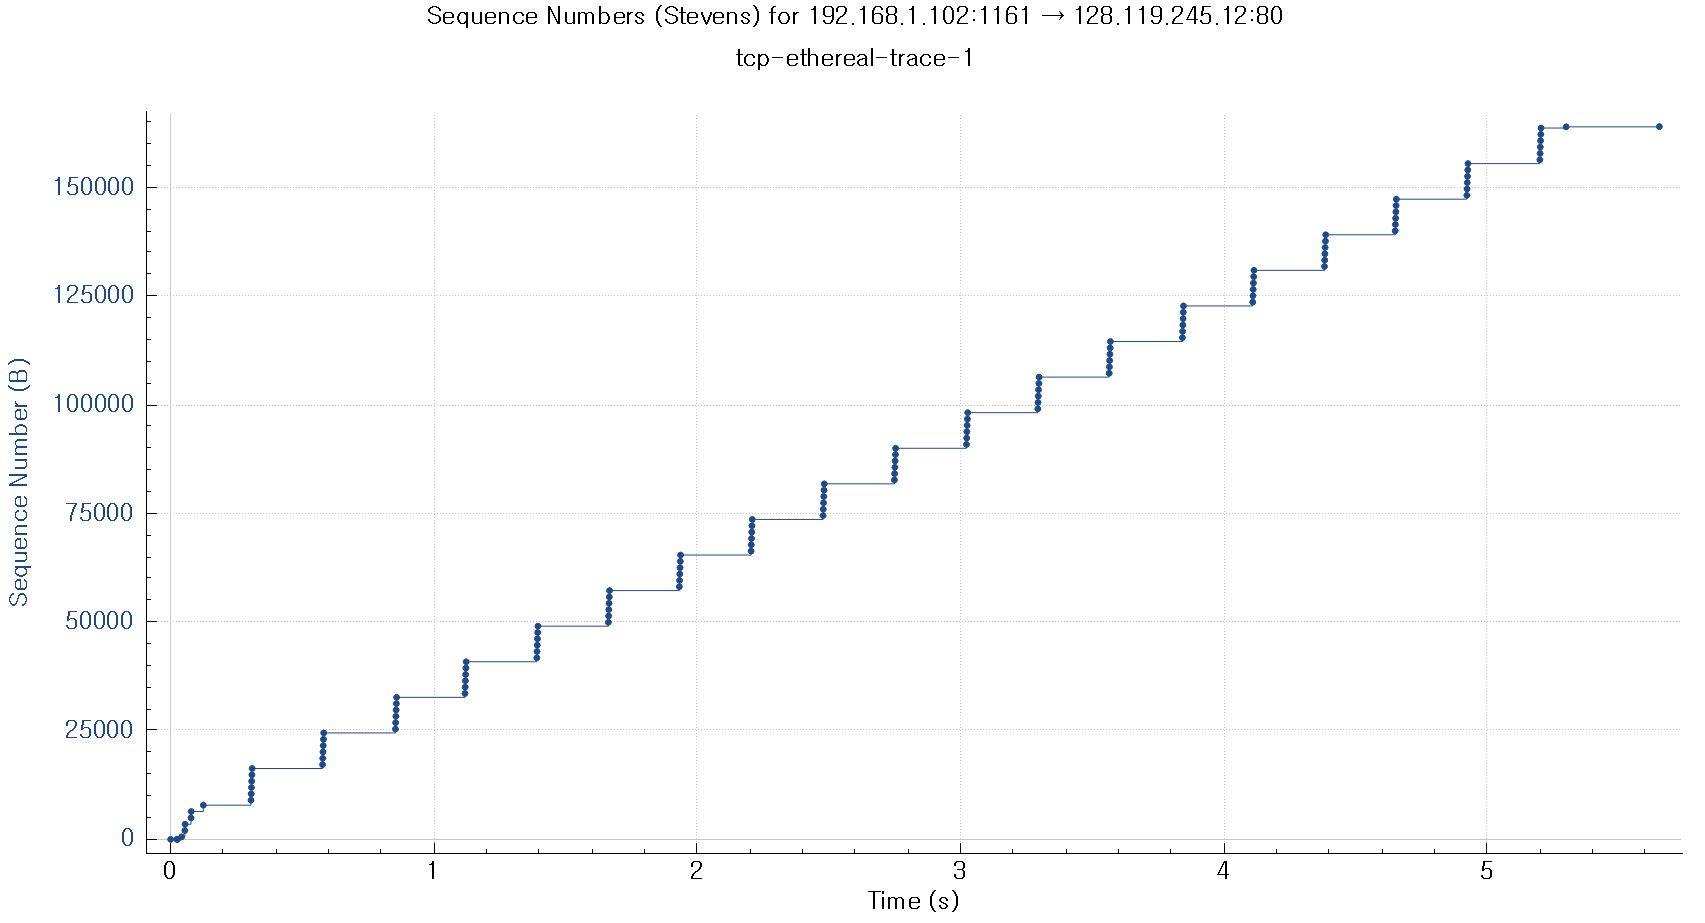
\includegraphics[width=.85\textwidth]{image/week02/1-9-1.png}
    		\caption{\footnotesize Problem 1-12's screenshot : }
    		\vspace{-10pt}
        \end{figure}
    \end{enumerate}
\newpage